\section{Espacios recubridores}

\begin{ejercicio}
    Sea $R=\left]-1,1\right[\subset \mathbb{R}$. Demuestra que existe una aplicación recubridora $p:R\to \mathbb{S}^1$. ¿Se puede levantar al recubridor la aplicación $f:\mathbb{S}^1\to\mathbb{S}^1$ dada por $f(x,y) = (y,x)$?\\

    \noindent
    Sabemos que $R$ es homeomorfo a $\mathbb{R}$ y que la aplicación $p_0:\mathbb{R}\to\mathbb{S}^1$ dada por:
    \begin{equation*}
        p_0(x) = (\cos(2\pi x), \sen(2\pi x))
    \end{equation*}
    es una aplicación recubridora. Si tomamos $h:R\to \mathbb{R}$ cualquier homeomofismo tendremos entonces que $p=p_0\circ h:R\to\mathbb{S}^1$ es una aplicación recubridora (como vimos en el Tema 1). En vistas del segundo apartado daremos $h$ de forma explícita, como por ejemplo:
    \begin{equation*}
        h(t) = \tg\left(\frac{\pi}{2}t\right)
    \end{equation*}
    Si consideramos la aplicación $f$ enunciada, estamos en la siguiente situación:
    \begin{figure}[H]
        \centering
        \shorthandoff{""}
        \begin{tikzcd}
                                        & R \arrow[d, "p"] \\
            \mathbb{S}^1 \arrow[r, "f"] & \mathbb{S}^1    
        \end{tikzcd}
        \shorthandon{""}
    \end{figure}
    \noindent
    Fijado $x_0 = (0,1)\in \mathbb{S}^1$, tomamos $b_0 = f(x_0) = (1,0)$ y $r_0 = 0\in p^{-1}(b_0)$. Tenemos que existe un levantamiento $\hat{f}:\mathbb{S}^1\to R$ de $f$ con $\hat{f}(x_0) = r_0$ si y solo si:
    \begin{equation}\label{eq:ej1_rel3}
        f_\ast(\pi_1(\mathbb{S}^1,(0,1))) \subseteq p_\ast(\pi_1(R,0))
    \end{equation}
    Pero tenemos que:
    \begin{equation*}
        \pi_1(R,0) = \{[\varepsilon_0]\} \quad\Longrightarrow\quad p_\ast(\pi_1(R,0)) = \{[\varepsilon_{(1,0)}]\}
    \end{equation*}
    $f_\ast$ es un isomorfismo por ser $f$ un homeomorfismo, por lo que:
    \begin{equation*}
        \pi_1(\mathbb{S}^1,(0,1))\cong \mathbb{Z} \quad\Longrightarrow\quad f_\ast(\pi_1(\mathbb{S}^1,(0,1))) \cong \mathbb{Z}
    \end{equation*}
    como no se puede cumplir la ecuación~\eqref{eq:ej1_rel3} tenemos que no existe dicho levantamiento. El mismo razonamiento puede repetirse para todo punto $x_0\in \mathbb{S}^1$.
\end{ejercicio}

\begin{ejercicio} 
    Dada la aplicación recubridora estándar $p:\mathbb{R}\to\mathbb{S}^1$ definida por
    \begin{equation*}
        p(x) = (\cos(2\pi x), \sen(2\pi x)),
    \end{equation*}
    determina si la aplicación $f:\mathbb{S}^1\to\mathbb{S}^1$ dada por $f(x,y) = (x,|y|)$ puede ser levantada al recubridor. Y, en tal caso, calcula sus levantamientos.\\

    \noindent
    Fijado $x_0=(1,0)\in \mathbb{S}^1$, tomamos $b_0 = f(x_0) = (1,0)$ y consideramos el punto $r_0=0\in p^{-1}(b_0)$. Existirá un levantamiento $\hat{f}:\mathbb{S}^1\to \mathbb{R}$ de $f$ con $\hat{f}(x_0) = r_0$ si y solo si:
    \begin{equation*}
        f_\ast(\pi_1(\mathbb{S}^1,x_0)) \subseteq p_\ast(\pi_1(\mathbb{R},r_0))
    \end{equation*}
    Tenemos que:
    \begin{equation*}
        \pi_1(\mathbb{R},r_0) = \{[\varepsilon_{r_0}]\} \quad\Longrightarrow\quad p_\ast(\pi_1(\mathbb{R},r_0)) = \{[\varepsilon_{b_0}]\}
    \end{equation*}
    Por otra parte, $\pi_1(\mathbb{S}^1,x_0)$ está generado por $[\alpha]$, con $\alpha:[0,1]\to \mathbb{S}^1$ dado por:
    \begin{equation*}
        \alpha(t) = (\cos(2\pi t), \sen(2\pi t))
    \end{equation*}

    y tenemos que:
    \begin{equation*}
        f_\ast([\alpha]) = [f\circ \alpha] 
    \end{equation*}

    donde:
    \begin{equation*}
        (f\circ \alpha)(t) = (\cos(2\pi t), |\sen(2\pi t)|)
    \end{equation*}
    que claramente es un arco homotópico a $\varepsilon_{b_0}$, por lo que tenemos:
    \begin{equation*}
        f_\ast(\pi_1(\mathbb{S}^1,x_0)) = \{[\varepsilon_{b_0}]\}
    \end{equation*}
    De donde existe una única $\hat{f}:\mathbb{S}^1\to \mathbb{R}$ aplicación continua con $\hat{f}(x_0) = r_0$. % // TODO: Calcular levantamiento
\end{ejercicio}

\begin{ejercicio}
    ¿Existe una aplicación recubridora desde $\mathbb{S}^1\times \mathbb{S}^1$ en $\mathbb{S}^1$?\\

    \noindent
    No: por reducción al absurdo, si existiera una aplicación recubridora $p:\mathbb{S}^1\times \mathbb{S}^1\to \mathbb{S}^1$:
    \begin{description}
        \item [Opción 1.] Tendríamos entonces por el Teorema de Monodromía que la aplicación $p$ induce un homomorfismo inyectivo $p_\ast:\pi_1(\mathbb{S}^1\times \mathbb{S}^1,x_0)\to \pi_1(\mathbb{S}^1,p(x_0))$ con $\pi_1(\mathbb{S}^1\times \mathbb{S}^1,x_0)\cong \mathbb{Z}\times \mathbb{Z}$ y $\pi_1(\mathbb{S}^1,p(x_0))\cong \mathbb{Z}$. Sin embargo, ningún subgrupo de $\mathbb{Z}$ es isomorfo a $\mathbb{Z}\times \mathbb{Z}$, por lo que llegamos a una contradicción.
        \item [Opción 2.] $\mathbb{R}$ es el recubridor universal de $\mathbb{S}^1$, por lo que entonces este también recubre a $\mathbb{S}^1\times \mathbb{S}^1$, y $\mathbb{R}^2$ también es recubridor universal de $\mathbb{S}^1\times \mathbb{S}^1$, por lo que ha de existir un isomorfismo de recubridores (y por tanto, un homeomorfismo) entre $\mathbb{R}$ y $\mathbb{R}^2$, algo imposible, pues $\mathbb{R}$ menos un punto no es conexo y $\mathbb{R}^2$ menos un punto sí lo es.
    \end{description}
\end{ejercicio}

\begin{ejercicio}
    Determina, salvo isomorfismos, todos los recubridores del cilindro $\mathbb{S}^1\times \mathbb{R}$.\\

    \noindent
    Fijado $b_0 = (1,0,0)\in \mathbb{S}^1\times \mathbb{R}$, tenemos que $\pi_1(\mathbb{S}^1\times \mathbb{R},b_0)\cong \mathbb{Z}$, y los subgrupos de $\mathbb{Z}$ son:
    \begin{equation*}
        H_k = k\mathbb{Z} \qquad k \in \mathbb{N}\cup \{0\}
    \end{equation*}
    \begin{itemize}
        \item Asociado a $H_0 = \{0\}$ tenemos el recubridor $(\mathbb{R}^2,p)$, donde $p = p_0\times Id_\mathbb{R}$, con $p_0:\mathbb{R}\to \mathbb{S}^1$ la aplicación recubridora estándar.
        \item Asociado a $H_k$ con $k\geq 1$ tenemos el recubridor $(\mathbb{S}^1\times \mathbb{R}, p_k)$, con la aplicación recubridora $p_k:\mathbb{S}^1\times \mathbb{R}\to \mathbb{S}^1\times \mathbb{R}$ dada por:
            \begin{equation*}
                p_k(\cos\theta, \sen\theta, y) = (\cos(k\theta), \sen(k\theta), y)
            \end{equation*}
    \end{itemize}
\end{ejercicio}

\begin{ejercicio} % // TODO: HACER
    Demuestra que si $p:R\to B$ es un homeomorfismo local con $R$ compacto y $B$ Hausdorff (y conexo), entonces $p$ es una aplicación recubridora.\\

    \noindent
    Recordamos que si $p$ es un homeomorfismo local entonces es una aplicación continua de forma que para cada punto $x\in R$ existe un abierto $U_x$ entorno de $x$ de forma que $p(U_x)$ es abierto en $B$ y $p\big|_{U_x}:U_x\to p(U_x)$ es un homeomorfismo.

    \begin{itemize}
        \item Tenemos que $p$ es continua por ser un homeomorfismo local.
        \item Como $R$ es compacto y $B$ es Hausdorff tenemos que $p$ es cerrada.
        \item Sea $U\subseteq R$ un abierto, podemos escribir:
            \begin{equation*}
                U = \bigcup_{x\in U}U_x
            \end{equation*}
            de donde $U_x\cap U$ es un abierto para cada $x\in U$, por lo que
            \begin{equation*}
                U = \bigcup_{x\in U} U_x \cap U
            \end{equation*}
            Para cada $x\in X$ tenemos que $p\big|_{U_x}:U_x\to p(U_x)$ es un homeomorfismo, por lo que $p(U_x\cap U)$ es un abierto de $B$. Finalmente, vemos:
            \begin{equation*}
                p(U) = p\left(\bigcup_{x\in U} U_x\cap U\right) = \bigcup_{x\in U} p(U_x\cap U)
            \end{equation*}
            Por lo que $p(U)$ es abierto, de donde $p$ es una aplicación abierta.
    \end{itemize}
    Como $p$ es abierta y cerrada tenemos que $p(R)\subseteq B$ es abierto y cerrado, como $B$ es conexo ha de ser $p(R) = B$, por lo que $p$ es sobreyectiva. Falta probar que todo punto $b\in B$ tiene un entorno abierto regularmente recubierto. % // TODO:
\end{ejercicio}

\begin{ejercicio} % // TODO: HACER
    Sea $p:\mathbb{R}^n\to \mathbb{R}^n$ un homeomorfismo local tal que para todo $r>0$ se tiene que $p^{-1}(\overline{B}(0,r))$ es compacto. Demuestra que $p$ es un homeomorfismo.
\end{ejercicio}

\begin{ejercicio}
    Sea $X$ conexo y localmente arcoconexo con grupo fundamental finito. Si $f,g:X\to \mathbb{R}$ son aplicaciones continuas cumpliendo que $f(x)^2 + g(x)^2 = 1$ para todo $x\in X$. Prueba que existe $h:X\to\mathbb{R}$ continua tal que $\cos(h(x)) = f(x)$ y $\sen(h(x)) = g(x)$ para cada $x\in X$.\\

    \noindent
    Observando la condición que cumplen $f$ y $g$ así como de la presencia de senos y cosenos pensamos en que el problema está relacionado con una circunferencia. Definimos por tanto $F:X\to \mathbb{S}^1$ dada por:
    \begin{equation*}
        F(x) = (f(x),g(x))
    \end{equation*}
    que está bien definida, pues $f(x)^2+g(x)^2 = 1$, por lo que $F(x)\in \mathbb{S}^1$ para todo $x\in X$. Si consideramos la aplicación recubridora estándar $p_0:\mathbb{R}\to \mathbb{S}^1$, fijado $x_0\in X$, $b_0 = F(x_0)$ y tomando $r_0\in p^{-1}(b_0)$ tenemos que existe un levantamiento $\hat{F}:X\to \mathbb{R}$ de $F$ con $\hat{F}(x_0) = r_0$ si y solo si:
    \begin{equation*}
        F_\ast(\pi_1(X,x_0)) \subseteq p_\ast(\pi_1(\mathbb{R},r_0))
    \end{equation*}
    Por una parte:
    \begin{equation*}
        \pi_1(\mathbb{R},r_0) = \{[\varepsilon_{r_0}]\} \quad\Longrightarrow\quad p_\ast(\pi_1k(\mathbb{R},r_0)) = \{[\varepsilon_{b_0}]\}
    \end{equation*}
    Por otra tenemos que como $\pi_1(X,x_0)$ es un grupo finito ha de ser por tanto $F_\ast(\pi_1(X,x_0))$ un subgrupo finito de $\pi_1(\mathbb{S}^1,b_0)\cong \mathbb{Z}$, que solo tiene un subgrupo finito, $\{[\varepsilon_{b_0}]\}$, de donde deducimos que ha de ser $F_\ast(\pi_1(X,x_0)) = \{[\varepsilon_{b_0}]\}$. Sea por tanto $\hat{F}:X\to \mathbb{R}$ el único levantamiento de $F$ con $\hat{F}(x_0) = r_0$, tenemos que:
    \begin{equation*}
        (\cos(2\pi \hat{F}(x)), \sen(2\pi \hat{F}(x))) = p(\hat{F}(x)) = F(x) = (f(x),g(x)) \qquad \forall x\in X
    \end{equation*}
    Por lo que si definimos $h:X\to \mathbb{R}$ dada por $h(x) = 2\pi \hat{F}(x)$, tenemos que:
    \begin{equation*}
        (\cos(h(x)), \sen(h(x))) = F(x) = (f(x),g(x)) \qquad \forall x\in X
    \end{equation*}
\end{ejercicio}

\begin{ejercicio} 
    Sean $p:X\to Y$ y $f:Y\to Z$ dos aplicaciones continuas tales que $p$ y $f\circ p$ son aplicaciones recubridoras. Prueba que $f$ es también una aplicación recubridora.\\

    \noindent
    Como $f\circ p$ es una aplicación recubridora es en particular sobreyectiva, por lo que $f$ también es sobreyectiva. Basta ver que para todo $z\in Z$ existe un entorno abierto de $z$ regularmente recubierto. Fijado $z\in Z$, tomamos $O_z$ un entorno abierto y arcoconexo de $z$ regularmente recubierto por la aplicación recubridora $f\circ p$, por lo que:
    \begin{equation*}
        p^{-1}(f^{-1}(O_z)) = (f\circ p)^{-1}(O_z) = \biguplus_{i \in I}A_i
    \end{equation*}
    con $A_i\subseteq X$ abierto y $(f\circ p)\big|_{A_i}:A_i\to O_z$ homeomorfismo para cada $i \in I$. Si aplicamos $p$ a dicha igualdad, obtenemos que:
    \begin{equation*}
        \bigcup_{i \in I}p(A_i) = p\left(\bigcup_{i \in I}A_i\right) = p(p^{-1}(f^{-1}(O_z))) \AstIg f^{-1}(O_z)
    \end{equation*}
    donde en $(\ast)$ hemos usado que $p$ es sobreyectiva, y tenemos además que $p(A_i)$ es abierto para cada $i \in I$, ya que $p$ es una aplicación abierta por ser una aplicación recubridora.\\

    \noindent
    Veamos ahora que si $p(A_i)\cap p(A_j)\neq \emptyset  \Longrightarrow p(A_i) = p(A_j)$: sea $y \in p(A_i)\cap p(A_j)$ existen entonces $x_i \in A_i$, $x_j \in A_j$ de forma que $p(x_i) = y = p(x_j)$, basta demostrar que $p(A_i)\subseteq p(A_j)$ y la otra inclusión será análoga. Para ello, sea $y'\in p(A_i)$, tenemos que existe $x'\in A_i$ de forma que $p(x') = y'$. Tomamos ahora $w=f(y), w'=f(y')$ y tendremos que $w,w'\in O_z$. Como $O_z$ es arcoconexo, existirá $\gamma:[0,1]\to Z$ de forma que $\gamma(0) = w$, $\gamma(1) = w'$. Si tomamos como $\hat{\gamma}$ el único levantamiento de $\gamma$ por $f\circ p$ con $\hat{\gamma}(0) = x_i$, como $Im \hat{\gamma}$ es un conjunto conexo ha de ser $Im \hat{\gamma}\subseteq A_i$ y como $(f\circ p)\big|_{A_i}:A_i\to O_z$ es un homeomorfismo, ha de ser $\hat{\gamma}(1) = x'$, ya que $(f\circ p)^{-1}(\{w'\})\cap A_i = \{x'\}$.\\

    \noindent
    Si consideramos ahora $\delta = p\circ \hat{\gamma}$ tenemos que:
    \begin{equation*}
        \delta(0) = p(x_i) = y, \qquad \delta(1) = p(x') = y'
    \end{equation*}
    y consideramos como $\hat{\delta}$ el único levantamiento de $\delta$ por $p$ con $\hat{\delta}(0) = x_j$. Tendremos:
    \begin{equation*}
        (f\circ p)\circ \hat{\delta} = f\circ \delta = f\circ p \circ \hat{\gamma} = \gamma
    \end{equation*}
    Por lo que $\hat{\delta}$ es el único levantamiento de $\gamma$ por $f\circ p$ con $\hat{\delta}(0) = x_j \in A_j$. Tendrá que ser $Im \hat{\delta}\subseteq A_j$, luego $\hat{\delta}(1)\in A_j$ y tenemos que:
    \begin{equation*}
        p(\hat{\delta}(1)) = \delta(1) = y'
    \end{equation*}
    por lo que $y'\in p(A_j)$, como queríamos probar. De esta forma, si eliminamos de la unión:
    \begin{equation*}
        \bigcup_{i \in I}p(A_i)
    \end{equation*}
    los conjuntos repetidos, obtendremos una unión disjunta, luego será:
    \begin{equation*}
        f^{-1}(O_z) = \biguplus_{j \in J}p(A_j)
    \end{equation*}
    y como $(f\circ p)\big|_{A_j}:A_j\to O_z$ es un homeomorfismo para cada $j \in J$ tenemos que:
    \begin{equation*}
        (f\circ p)\big|_{A_j} = f\big|_{p(A_j)} \circ p\big|_{A_j}
    \end{equation*}
    Por lo que $f\big|_{p(A_j)}:A_j\to O_z$ es inyectiva y con todas las demás propiedades que hemos probado de $f$ deducimos que $f\big|_{p(A_j)}:p(A_j)\to O_z$ es un homeomorfismo para cada $j\in J$. En definitiva, hemos probado que la aplicación $f$ es una aplicación recubridora.
\end{ejercicio}

\begin{ejercicio}
    Sean $p_1:X\to Y$ y $p_2:Y\to Z$ dos aplicaciones recubridoras. Prueba que si $Z$ tiene recubridor universal, entonces $p_2\circ p_1:X\to Z$ es una aplicación recubridora.\\

    \noindent
    Si $Z$ tiene recubridor universal $(R,p)$ tenemos que como $(Y,p_2)$ también recubre a $Z$ existirá entonces un homomorfismo de recubridores $\phi_1$ de $(R,p)$ en $(Y,p_2)$, por lo que $R$ es recubridor universal de $Y$. Repetiendo el razonamiento con el recubridor $(X,p_1)$ de $Y$ tenemos que existe un homomorfismo de recubridores $\phi_2$ de $(R,p)$ en $(X,p_1)$, obteniendo que el siguiente diagrama es conmutativo:
    \begin{figure}[H]
        \centering
        \shorthandoff{""}
        \begin{tikzcd}
                               &                    & R \arrow[d, "p"] \arrow[ld, "\phi_1", bend right] \arrow[lld, "\phi_2", bend right] \\
            X \arrow[r, "p_1"] & Y \arrow[r, "p_2"] & Z                                                                                  
        \end{tikzcd}
        \shorthandon{""}
    \end{figure}
    \noindent
    De esta forma, tenemos que:
    \begin{equation*}
        (p_2\circ p_1)\circ \phi_2 = p
    \end{equation*}
    con $\phi_2$ y $p$ aplicaciones recubridoras, por lo que por el ejercicio anterior tenemos que $p_2\circ p_1$ es una aplicación recubridora.
\end{ejercicio}

\begin{ejercicio}
    Sean $p:R\to B$ una aplicación recubridora y $b_0\in B$. Definimos la aplicación (correspondencia del levantamiento generalizada)
    \Func{\phi}{p^{-1}(\{b_0\})\times \pi_1(B,b_0)}{p^{-1}(\{b_0\})}{(r,[\alpha])}{\hat{\alpha}_r(1)}
    donde $\hat{\alpha}_r(s)$ es el único levantamiento de $\alpha(s)$ con condición inicial $\hat{\alpha}_r(0)=r$. Demuestra que:
    \begin{enumerate}[label=\alph*)]
        \item $\phi$ está bien definida.

            Fijado $r\in p^{-1}(b_0)$ tenemos que la aplicación correspondencia del levantamiento 
            \Func{\phi_r}{\pi_1(B,b_0)}{p^{-1}(\{b_0\})}{[\alpha]}{\hat{\alpha}(1)}
            donde $\hat{\alpha}$ es el único levantamiento de $\alpha$ con condición inicial $\hat{\alpha}(0) = r$ está bien definida, por lo que $\phi$ estará bien definida.
        \item $\phi(r,[\varepsilon_{b_0}])=r$, para cualquier $r\in p^{-1}(\{b_0\})$.

            Sea $r\in p^{-1}(\{b_0\})$, si consideramos $\varepsilon_{r}$ tenemos que:
            \begin{equation*}
                p\circ \varepsilon_r = \varepsilon_{b_0}, \qquad \varepsilon_r(0) = r
            \end{equation*}
            Por lo que $\varepsilon_r$ es el único levantamiento de $\varepsilon_{b_0}$ con $\varepsilon_r(0) = r$, de donde ha de ser:
            \begin{equation*}
                \phi_r(r,[\varepsilon_{b_0}]) = \varepsilon_r(1) = r
            \end{equation*}
        \item $\phi(\phi(r,[\alpha]),[\beta]) = \phi(r,[\alpha]\ast[\beta])$, para cualesquiera $r\in p^{-1}(\{b_0\})$ y $[\alpha],[\beta]\in \pi_1(B,b_0)$.

            Sea $\hat{\alpha}_r$ el único levantamiento de $\alpha$ con $\hat{\alpha}_r(0) = r$ tenemos entonces que $\phi(r,[\alpha]) = \hat{\alpha}_r(1) = r_1\in p^{-1}(\{b_0\})$. Sea $\hat{\beta}_{r_1}$ el único levantamiento de $\beta$ con $\hat{\beta}_{r_1}(0) = r_1$, tenemos que $\phi(r_1,[\beta]) = \hat{\beta}_{r_1}(1)$.

            Veamos finalmente que $\hat{\alpha}_r\ast \hat{\beta}_{r_1}$ es un levantamiento de $\alpha\ast\beta$, que además cumple:
            \begin{equation*}
                (\hat{\alpha}_r\ast\hat{\beta}_{r_1})(0) = \hat{\alpha}_r(0) = r
            \end{equation*}
            Para ello, vemos que:
            \begin{align*}
                p((\hat{\alpha}_r\ast\hat{\beta}_{r_1})(t)) &= p\left(
                \left\{\begin{array}{ll}
                        \hat{\alpha}_r(2t) & \text{si\ } 0\leq t\leq \nicefrac{1}{2} \\ 
                        \hat{\beta}_{r_1}(2t-1) & \text{si\ } \nicefrac{1}{2}\leq t\leq 1
                \end{array}\right. \right) \\
                            &= \left\{\begin{array}{ll}
                                    p(\hat{\alpha}_r(2t)) & \text{si\ } 0\leq t\leq \nicefrac{1}{2} \\
                                    p(\hat{\beta}_{r_1}(2t-1)) & \text{si\ } \nicefrac{1}{2}\leq t\leq 1
                                    \end{array}\right.  \\ &= \left\{\begin{array}{ll}
                                \alpha(2t) & \text{si\ } 0\leq t\leq\nicefrac{1}{2} \\
                                \beta(2t-1) & \text{si\ } \nicefrac{1}{2}\leq t\leq 1
                            \end{array}\right.  = (\alpha\ast \beta)(t)
            \end{align*}
            Por lo que ha de ser:
            \begin{equation*}
                \phi(r,[\alpha]\ast [\beta]) = \phi(r,[\alpha\ast \beta]) = (\hat{\alpha}_r\ast\hat{\beta}_{r_1})(1) = \hat{\beta}_{r_1}(1) = \phi(\phi(r,[\alpha]),[\beta])
            \end{equation*}
        \item $\phi$ es sobreyectiva.

            En efecto, sea $r\in p^{-1}(b_0)$, tenemos que $\phi(r,[\varepsilon_{b_0}]) = r$.
        \item $\phi(r,[\alpha]) = r$ si y solo si $[\alpha] \in p_\ast(\pi_1(R,r))$.
            Por doble implicación:
            \begin{description}
                \item [$\Longleftarrow )$] Si $[\alpha]\in p_\ast(\pi_1(R,r))$ tenemos entonces que existe $[\beta]\in \pi_1(R,r)$ de forma que $[p\circ \beta] = p_\ast([\beta]) = [\alpha]$, por lo que $\beta$ es un levantamiento de $\alpha$, que además cumple $\beta(0) = r$, por lo que:
                    \begin{equation*}
                        \phi(r,[\alpha]) = \hat{\alpha}_r(0) = \beta(0) = r
                    \end{equation*}
                \item [$\Longrightarrow )$] Si $\phi(r,[\alpha]) = r$ tenemos entonces que el único levantamiento $\hat{\alpha}_r$ de $\alpha$ con $\hat{\alpha}_r(0) = r$ es un lazo en $R$, $[\hat{\alpha}_r]\in \pi_1(R,r)$, y tenemos que $p_\ast([\hat{\alpha}_r]) = [\alpha]$ por ser $\hat{\alpha}_r$ levantamiento de $\alpha$.
            \end{description}
        \item El cardinal de $p^{-1}(\{b_0\})$ coincide con el cardinal de $\pi_1(B,b_0)/p_\ast(\pi_1(R,r))$ (es decir, el índice de $p_\ast(\pi_1(R,r))$ como subgrupo de $\pi_1(B,b_0)$). % // TODO: TERMINAR
    \end{enumerate}
\end{ejercicio}

\begin{ejercicio}\label{ej:11_rel3}
    Sea $X$ un espacio topológico (conexo y localmente arcoconexo), $G$ un grupo de homeomorfismos de $X$ y $X/\cc{R}_G$ el espacio topológico cociente dado por la relación de equivalencia:
    \begin{equation*}
        x\cc{R}_G y \quad\Longleftrightarrow\quad\exists \varphi \in G : y = \varphi(x)
    \end{equation*}
    para cualesquiera $x,y\in X$.\newline
    Demuestra que la aplicación proyección $\pi:X\to X/\cc{R}_G$ es recubridora si y solo si para cada $x\in X$ existe un entorno suyo $U_x$ tal que $\varphi(U_x)\cap U_x=\emptyset $ para todo $\varphi\in G\setminus \{Id_X\}$.\newline
    Deduce que, además, $\varphi:(X,\pi)\to (X,\pi)$ es un isomorfismo de recubridores si y solo si $\varphi \in G$.
\end{ejercicio}

\begin{ejercicio}
    Para cada $n\in \mathbb{Z}$ se define $f_n:\mathbb{R}^2\to\mathbb{R}^2$ como $f_n(x,y) = (x+2n,{(-1)}^{n}y)$. Utiliza el ejercicio anterior para demostrar que:
    \begin{enumerate}[label=\alph*)]
        \item $G = \{f_n:n\in \mathbb{Z}\}$ es un grupo de homeomorfismos de $\mathbb{R}^2$ y para cada $x\in \mathbb{R}^2$ existe un entorno suyo $U_x$ tal que $f_n(U_x)\cap U_x = \emptyset $ para todo $n\in \mathbb{Z}\setminus \{0\}$.
        \item La proyección $p:\mathbb{R}^2\to\mathbb{R}^2/\cc{R}_G$ es una aplicación recubridora de $\mathbb{R}^2$ en la cinta de Moebius $\mathbb{R}^2/\cc{R}_G$.
    \end{enumerate}
\end{ejercicio}

\begin{ejercicio}
    Para cada $n,m\in \mathbb{Z}$ se define $f_{n,m}:\mathbb{R}^2\to\mathbb{R}^2$ como:
    \begin{equation*}
        f_{n,m}(x,y) = (x,{(-1)}^{n}y) + 2(n,{(-1)}^{n}m).
    \end{equation*}
    Utiliza el ejercicio~\ref{ej:11_rel3} para demostrar que:
    \begin{enumerate}[label=\alph*)]
        \item $G=\{f_{n,m}:n,m\in \mathbb{Z}\}$ es un grupo de homeomorfismos de $\mathbb{R}^2$ y para cada $x\in \mathbb{R}^2$ existe un entorno suyo $U_x$ tal que $f_{n,m}(U_x)\cap U_x=\emptyset $ para todo $n,m\in \mathbb{Z}$ con $(n,m)\neq (0,0)$.
        \item La proyección $p:\mathbb{R}^2\to\mathbb{R}^2/\cc{R}_G$ es una aplicación recubridora de $\mathbb{R}^2$ en la botella de Klein $\mathbb{R}^2/\cc{R}_G$.
    \end{enumerate}
\end{ejercicio}

\begin{ejercicio}
    Razona si son verdaderas o falsas las siguientes afirmaciones:
    \begin{enumerate}[label=\alph*)]
        \item Existe una aplicación recubridora $p:\mathbb{S}^1\to [0,1]$.

            Es falsa, ya que si existiera una aplicación recubridora $p:\mathbb{S}^1\to [0,1]$ el Teorema de Monodromía nos diría que el homomorfismo inducido por la aplicación $p$ $p_\ast:\pi_1(\mathbb{S}^1,x_0)\to \pi_1([0,1],p(x_0))$ es inyectivo, con $\pi_1(\mathbb{S}^1,x_0)\cong \mathbb{Z}$ y $\pi_1([0,1],p(x_0)) = \{[\varepsilon_{x_0}]\}$, lo que llevaría a una contradicción.
        \item Existe una aplicación recubridora $p:\mathbb{R}\bb{P}^2\to \mathbb{S}^1$.

            Es falsa, ya que si existiera una aplicación recubridora $p:\mathbb{R}\bb{P}^2\to \mathbb{S}^1$:
            \begin{description}
                \item [Opción 1.] el Teorema de Monodromía nos diría que el homomorfismo inducido $p_\ast:\pi_1(\mathbb{R}\bb{P}^2,x_0)\to \pi_1(\mathbb{S}^1,p(x_0))$ es inyectivo, con $\pi_1(\mathbb{R}\bb{P}^2,x_0)\cong \mathbb{Z}_2$, pero entonces tenemos que $p_\ast(\pi_1(\mathbb{R}\bb{P}^2,x_0)) \cong \mathbb{Z}_2$ y subgrupo de $\pi_1(\mathbb{S}^1,p(x_0))\cong \mathbb{Z}$, que es una contradicción.
                \item [Opción 2.] Como $\mathbb{R}$ es el recubridor universal de $\mathbb{S}^1$ tendríamos entonces que $\mathbb{R}$ recubriría a $\mathbb{R}\bb{P}^2$, y el recubridor universal de $\mathbb{R}\bb{P}^2$ es $\mathbb{S}^2$, por lo que tendríamos entonces un homeomorfismo entre $\mathbb{R}$ y $\mathbb{S}^2$, algo imposible, pues $\mathbb{S}^2$ es compacto y $\mathbb{R}$ no.
            \end{description}
        \item El semiplano $X=\{(x,y)\in \mathbb{R}^2 : y\geq 0\}$ es el recubridor universal de la bola cerrada punteada $Y = \{(x,y)\in \mathbb{R}^2 : 0<x^2+y^2 \leq 1\}$.

            Es verdadera, es claro que $X$ es simplemente conexo, por lo que basta ver que existe alguna aplicación recubridora $p:X\to Y$.
            \begin{figure}[H]
                \centering
                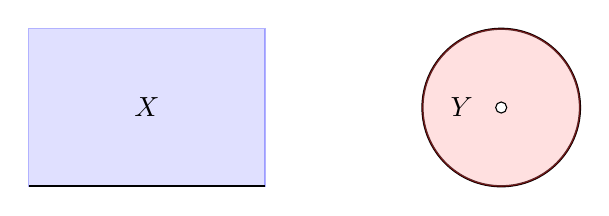
\begin{tikzpicture}
                    \filldraw[fill=blue!40, draw=blue, opacity=0.3] (0,0) rectangle (3,2);
                    \draw[thick] (0,0) -- (3,0);
                    \fill(1.5,1) node[] {$X$};
                    \draw[thick](6,1) circle(1cm);
                    \draw[fill = red!40, draw=red, opacity=0.3](6,1) circle(1cm);
                    \fill(5.5,1) node[] {$Y$};
                    \draw[fill=white] (6,1) circle (2pt);
                \end{tikzpicture}
            \end{figure}
            Sabemos ya de la existencia de una aplicación recubridora $p_0:\mathbb{R}\to \mathbb{S}^1$, por lo que sabemos llevarnos el ``borde'' de $X$ al ``borde'' de $Y$. Si repetimos el proceso subiendo la altura en $X$ y achicando el radio en $Y$ conseguiremos una aplicación recubridora $p:X\to Y$. La idea es buscar una aplicación que en $0$ valga $1$ y que su imagen tienda a $0$ en infinito. Tomamos por tanto $p:X\to Y$ dada por:
            \begin{equation*}
                p(x,y) = e^{-y}p_0(x)
            \end{equation*}
            \begin{figure}[H]
                \centering
                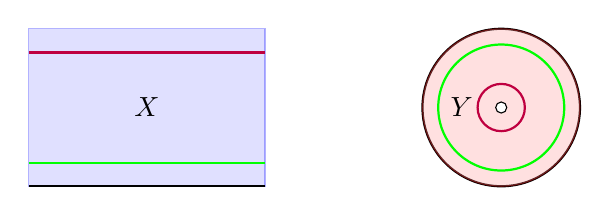
\begin{tikzpicture}
                    \filldraw[fill=blue!40, draw=blue, opacity=0.3] (0,0) rectangle (3,2);
                    \draw[thick] (0,0) -- (3,0);
                    \fill(1.5,1) node[] {$X$};
                    \draw[thick](6,1) circle(1cm);
                    \draw[fill = red!40, draw=red, opacity=0.3](6,1) circle(1cm);
                    \fill(5.5,1) node[] {$Y$};
                    \draw[fill=white] (6,1) circle (2pt);

                    \draw[thick, draw=green] (0,0.3) -- (3,0.3);
                    \draw[thick, draw=green] (6,1) circle(0.8cm);
                    \draw[thick, draw=purple] (0,1.7) -- (3,1.7);
                    \draw[thick, draw=purple] (6,1) circle(0.3cm);
                \end{tikzpicture}
            \end{figure}
            Es claro que $p$ es continua y sobreyectiva. Se comprueba además que $p$ es una aplicación recubridora.

        \item Si $X$ es un espacio topológico (conexo y localmente arcoconexo) con grupo fundamental finito y $p:X\to X$ es una aplicación recubridora, entonces $p$ es un homeomorfismo.

            Es verdadera. Para probar que $p$ es un homeomorfismo basta probar que $p$ es inyectiva, pues al ser una aplicación recubridora tenemos ya que es continua, sobreyectiva y abierta. Para ver que es inyectiva, tomamos dos puntos $x,y\in X$ con $p(x) = p(y)$, como $X$  es conexo y localmente arcoconexo vimos en el Tema 1 que entonces $X$ es arcoconexo, por lo que en particular ha de existir un arco $\alpha:[0,1]\to X$ de forma que $\alpha(0) = x$ y $\alpha(1) = y$. Si consideramos el arco $p\circ \alpha$ tenemos que:
            \begin{equation*}
                (p\circ \alpha)(0) = p(x) = p(y) = (p\circ \alpha)(1)
            \end{equation*}
            por lo que $p\circ \alpha$ es un lazo en $X$. Por otra parte, el Teorema de Monodromía nos dice que el homomorfismo $p_\ast:\pi_1(X,x) \to \pi_1(X,p(x))$ es inyectivo, por lo que será un isomorfismo de grupos, al ser $\pi_1(X,x)$ finito. De esta forma, como $[p\circ \alpha] \in \pi_1(X,p(x))$, ha de existir $\beta\in \Omega(X,x)$ de forma que $p_\ast([\beta]) = [p\circ \alpha]$. En este momento tenemos que tanto $\beta$ como $\alpha$ son dos levantamientos de $p\circ \alpha$ con:
            \begin{equation*}
                \beta(0) = x = \alpha(0)
            \end{equation*}
            por lo que han de ser iguales, de donde:
            \begin{equation*}
                y = \alpha(1) = \beta(1) = x
            \end{equation*}
    \end{enumerate}
\end{ejercicio}
